\setlength{\tabcolsep}{1pt}
\begin{figure}[h]
    \footnotesize
    \small
    % \begin{tabular}{*{6}{p{2.8cm}}}
    %   \hline
    %   & & & & & \\
    %   \centering Input & \centering \ptopzero & \centering \nulltext & \centering  \directinversion & \centering  \negprox & \centering \method{} \\
    %   %   \multicolumn{6}{c}{``\textit{A \textcolor{RoyalBlue}{\textbf{lego}} cat \textcolor{RoyalBlue}{\textbf{toy}} sitting next to a mirror}"} \\
    %   \multicolumn{6}{c}{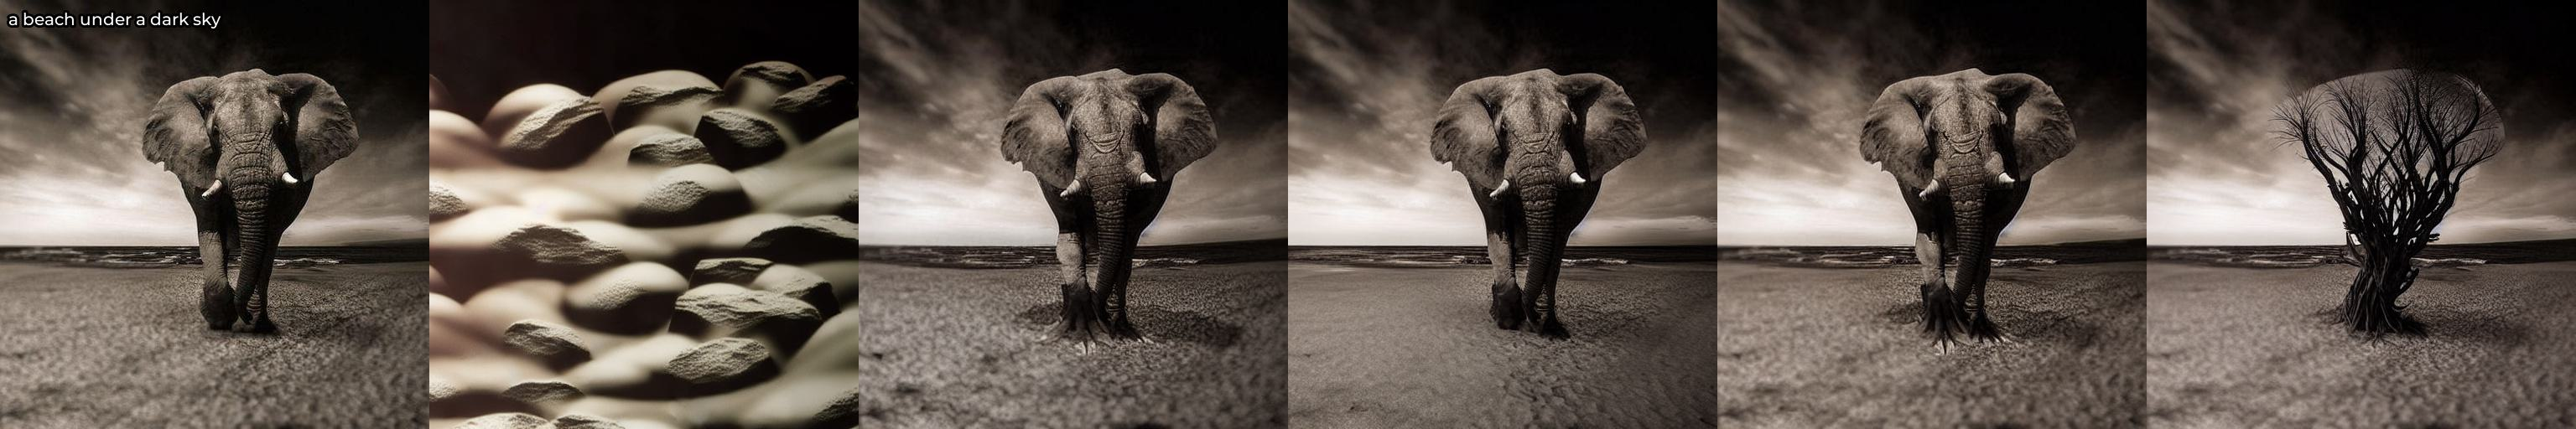
\includegraphics[width=\linewidth]{fig/ex_structpres/3_delete_object_80-2_natural-1_animal-321000000005}} \\
    % \multicolumn{6}{c}{}  \\
    % % 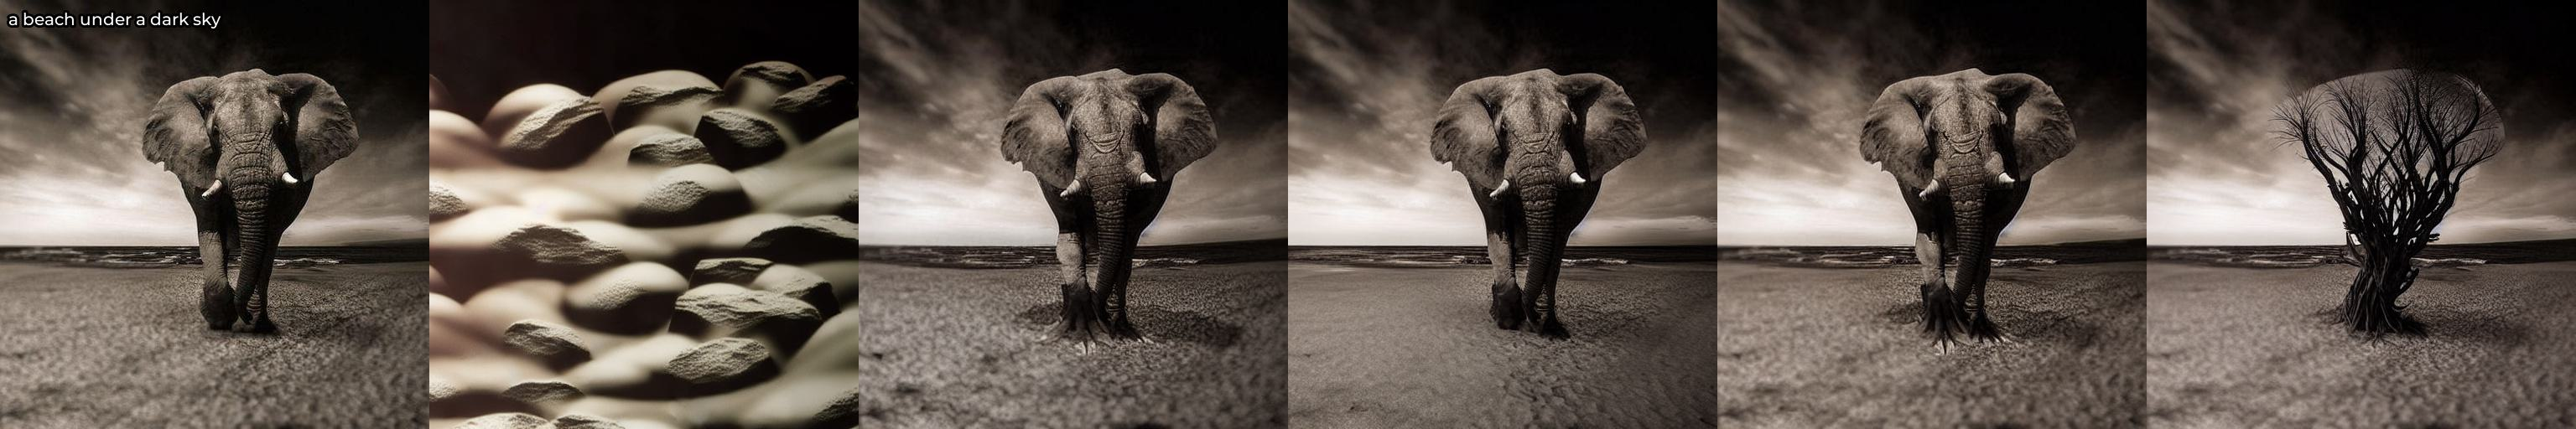
\includegraphics[height=2.2cm]{fig/ex_structpres/3_delete_object_80-2_natural-1_animal-321000000005} \\
    % %   \multicolumn{6}{c}{``\textit{Orange van with \textcolor{BrickRed}{\st{surfboards}} \textcolor{RoyalBlue}{\textbf{flowers}} on top}"} \\
    % %   \insertimage{van}{input}\\
    % %   \multicolumn{6}{c}{``\textit{Meat \textcolor{BrickRed}{\st{balls}} \textcolor{RoyalBlue}{\textbf{shushi}} on white plate}"} \\
    % %   \insertimage{meat}{input}\\
    % %   \multicolumn{6}{c}{``\textit{A \textcolor{BrickRed}{\st{woman}} \textcolor{RoyalBlue}{\textbf{storm-trooper}} with blue hair}"} \\
    % %   \insertimage{girl}{input}\\
    % %   \multicolumn{6}{c}{``\textit{A \textcolor{BrickRed}{\st{cat}} \textcolor{RoyalBlue}{\textbf{dog}} sitting on a wooden chair}"} \\
    % %   \insertimage{cat2}{input}\\
    %   \hline
    %   % ... Add more rows as needed
    % \end{tabular}
    \begin{tabularx}{\columnwidth}{ YYYYYY }
        Input & \ptopzero &  \nulltext &  \directinversion &  \negprox &  \method \\
        \multicolumn{6}{c}{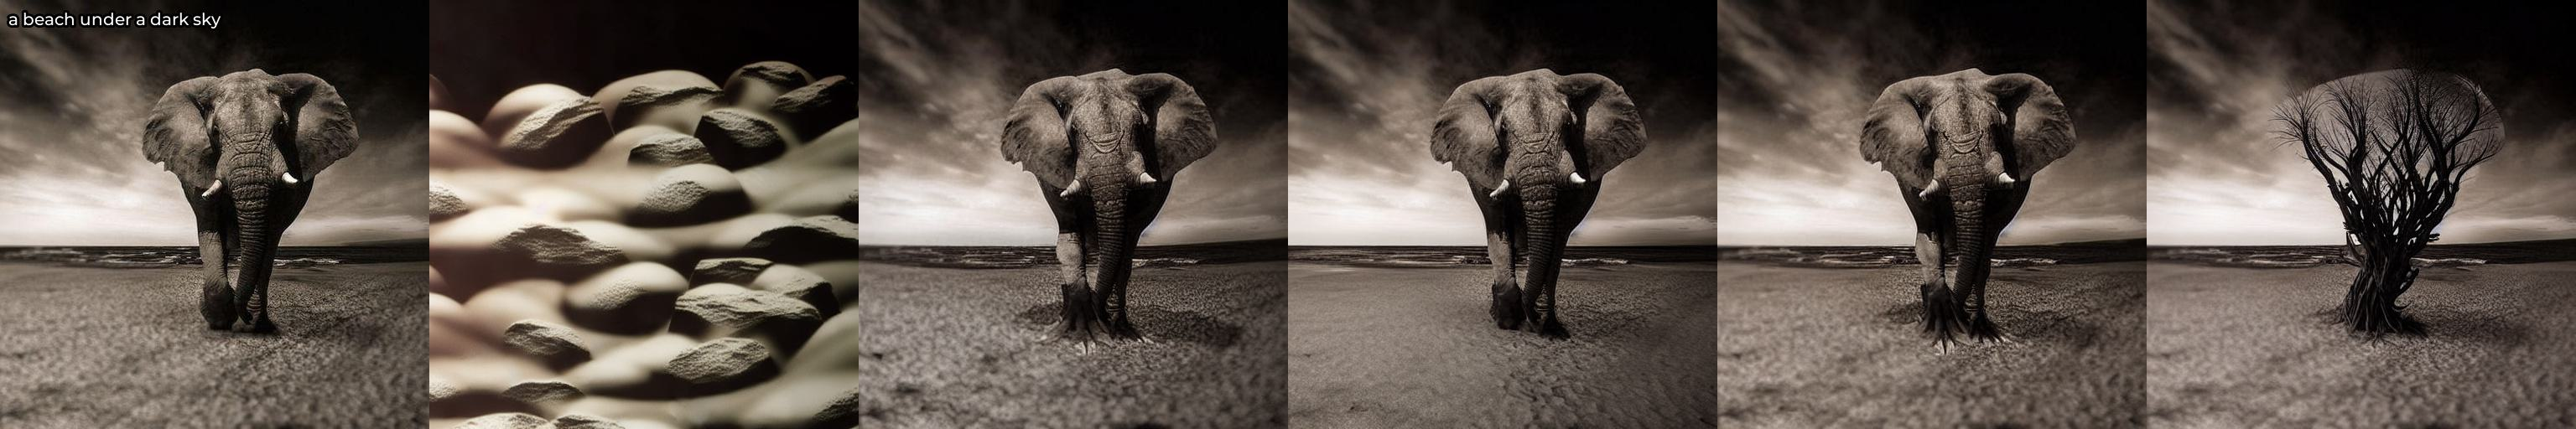
\includegraphics[width=\linewidth]{fig/ex_structpres/3_delete_object_80-2_natural-1_animal-321000000005}} \\
        \multicolumn{6}{c}{``\textit{\textcolor{BrickRed}{\st{an elephant walking on}} a beach under a dark sky}"} \\
        \multicolumn{6}{c}{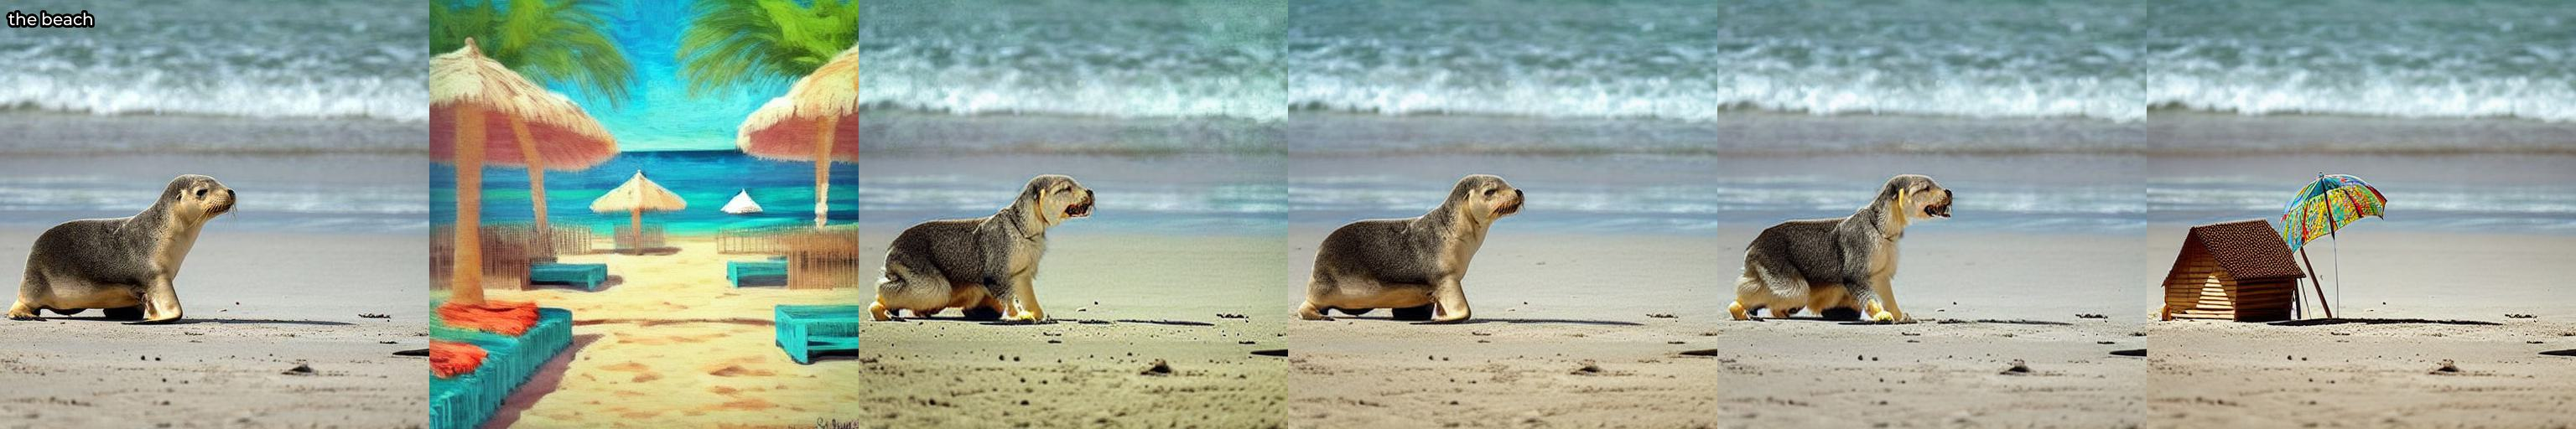
\includegraphics[width=\linewidth]{fig/ex_structpres/3_delete_object_80-2_natural-1_animal-321000000006}} \\
        \multicolumn{6}{c}{``\textit{\textcolor{BrickRed}{\st{a seal pup on}} the beach}"} \\
        
        \end{tabularx}
    % \caption{PieBench examples. STRUCTURE PRESERVATION.}
    \caption{Examples of object removal by \method{}. Although the method inadvertently fills gaps with structurally similar content, likely due to the complex interplay between CFG and self-attention guidance, it remains the only approach that consistently and effectively removes target objects.}
    \label{fig:sup_structpres}
  \end{figure}